\subsection{Citus: PostgreSQL Terdistribusi}

Citus merupakan mesin basis data terdistribusi (\textit{distributed database engine}) untuk PostgreSQL yang menangani kebutuhan skalabilitas pada ekosistem PostgreSQL \parencite{citus}. Sebagai sebuah ekstensi, Citus menjaga kompatibilitas dengan PostgreSQL, sehingga dapat digunakan dengan PostgreSQL versi terbaru.

Sebuah kluster memiliki banyak \textit{nodes} yang terspesialisasi menjadi koordinator dan node pekerja. Aplikasi mengirimkan \textit{query} kepada koordinator, lalu diteruskan kepada node pekerja terkait. Pendekatan ini memungkinkan setiap \textit{node} mampu memproses permintaan tulis sehingga pemrosesan bisa dilakukan secara parallel (\textit{multiple writer}).

Selain itu, berikut adalah fitur lain ekstensi Citus:

\begin{enumerate}
    \item Tabel dibagi ke seluruh kluster node untuk menggabungkan sumber daya mesin (\textit{distributed tables}).
    \item Tabel referensi direplikasi ke seluruh node untuk kebutuhan penggabungan (\textit{join}) dan \textit{foreign key}, sehingga kinerja pembacaan data semakin baik (\textit{references tables}).
    \item Mesin kueri terdistribusi mengarahkan dan memparalelkan operasi pada tabel terdistribusi ke seluruh kluster (\textit{Distributed query engine router}).
\end{enumerate}

Citus memiliki dua model pembagian data (\textit{sharding}), yaitu pembagian berdasarkan baris (\textit{row-based sharding}) dan pembagian berdasarkan skema (\textit{schema based sharding}).

\begin{figure}[htbp]
    \centering
    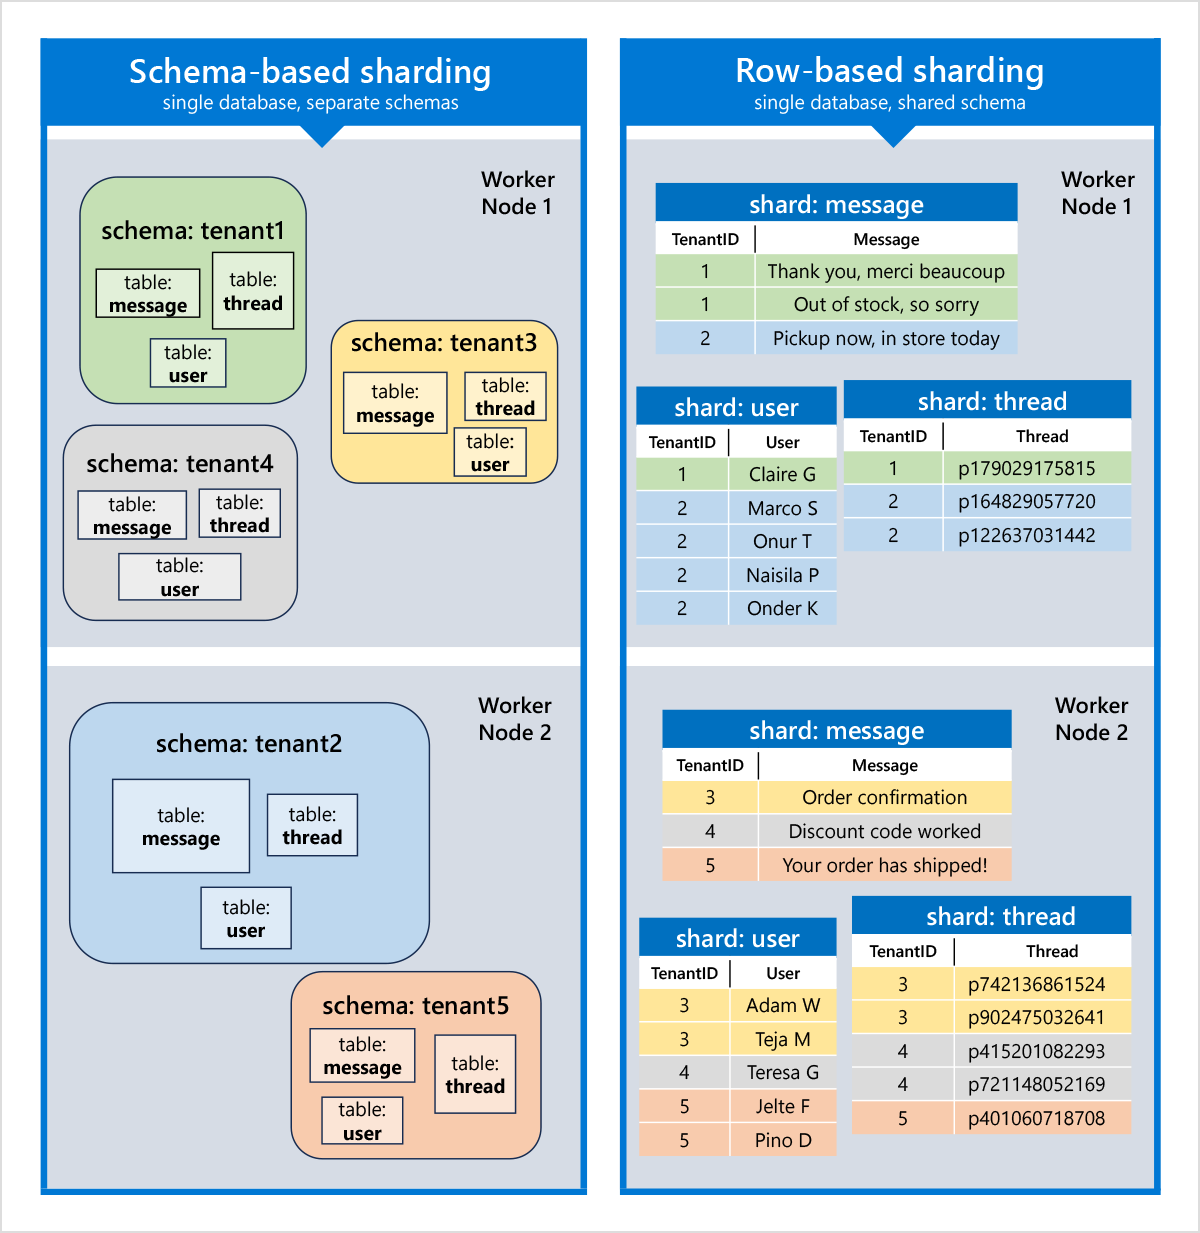
\includegraphics[width=0.8\textwidth]{resources/chapter-2/row-vs-schema-sharding.png}
    \caption{Perbandingan Pembagian Data Berdasarkan Baris dan Skema \parencite{schemaBasedSharding}}
    \label{fig:row-vs-schema-sharding}
\end{figure}

